%% -*- tex-main-file:"rcu-cc.tex" -*-

\section{Introduction}
\seclabel{intro}

%1. new hw trend has led to new systems
Modern systems with massively parallel processors and large main memories have inspired a new breed of high-performance, memory-optimized transaction processing systems \cite{Kallman+08,PandisJHA10,KemperN11,LarsonBDFPZ11,LevandoskiLSSW15,TuZKLM13}. These systems leverage spacious main memory to fit the whole working set in DRAM with streamlined, memory-friendly data structures. Further, optimizations for multicore and multi-socket hardware allow a much higher level of parallelism compared to conventional database systems. With disk overheads and delays removed, transaction latencies drop precipitously and worker threads can usually execute transactions to completion without interruption. The result is a welcome reduction in contention at the logical level and less pressure on whatever concurrency control (CC) scheme might be in place. A less welcome result is an increasing pressure for scalable data structures and algorithms to cope with the growing number of threads that concurrently execute transactions and need to communicate.

\labeledfigurewide{fig-write-ratio}{Performance of a memory-efficient OLTP engine with lightweight optimistic concurrency control, as the ratio of writes increases (left); and as the size of the database decreases (right).}

\vspace{2mm}
{\bf Interactions at the logical level.} 
%2. how current workloads make cc important again.
Many designs exploit the reduction in the pressure on CC, by employing very optimistic and lightweight schemes, boosting even further the performance of these systems on suitable workloads.
But, as is usually the case, it appears that database workloads stand ready to absorb any and all concurrency gains the memory-optimized systems have to offer. In particular, there is high demand for database systems that can readily serve heterogeneous database workloads, blending the gap between transaction and analytical processing. This trend is at least partly enabled by the improved concurrency and reduced contention offered by memory-optimized systems \cite{Farber+12}. Mixed workloads have two significant impacts on CC, however. First, the write/read ratio decreases from 1:2 (e.g. TPC-C) to 1:10 or less (e.g. TPC-E \cite{Chen+10,TozunPKJA13}), usually {\it by increasing the number of reads as the number of writes remains stable}.
Second, workloads frequently include some fraction of large transactions that are {\it read-mostly rather than read-only}---a trend reflected in the TPC-E benchmark. Unfortunately, both of these workload properties result in larger effective concurrency control footprints, putting pressure on the CC scheme. 
Therefore, going forward and as the industry shifts to heterogeneous workloads served by memory-optimized engines, it is vital for them to employ effective and robust CC schemes. 


We observe that the CC schemes currently in vogue with memory-optimized systems are not robust under contention, particularly when short write-intensive transactions coexist with longer \textit{read-mostly} transactions.
The two main families of approaches can be loosely classified as two-phase locking (2PL) and optimistic concurrency control (OCC). 2PL is common in traditional disk-oriented systems, and is often criticized because of high overheads, its policy of blocking transactions (leading to deadlocks and other scheduling problems), and a tendency to ``lock up'' (performance crash) once the aggregate transactional footprint grows too large, a state quickly attained when heavy read-mostly transactions enter the system. OCC, on the other hand, never blocks readers---and may not even block writers---thus avoiding most scheduling issues. Although they differ in details, the rising generation of memory-optimized systems almost universally adopts a form of OCC that is effectively single-versioned, with read footprint validation at pre-commit.  Two systems that characteristically employ this type of OCC are Microsoft's Hekaton \cite{LarsonBDFPZ11} and Silo \cite{TuZKLM13}. This type of approach suffers badly in highly concurrent workloads \cite{YuBPDS14} because transactions must abort if any portion of their read footprint is overwritten before they commit. 
In \figref{fig-write-ratio} we demonstrate how the performance of Silo, a representative of the camp of transaction processing engines with lightweight OCC, degrades as transactions have larger read footprint or when contention increases. (\secref{eval:setup} has details about the experimental setup.) \figref{fig-write-ratio}(left) shows that it just takes 0.1\% or 1\% of the touched records to be updates for the transaction throughput to drastically drop. While \figref{fig-write-ratio}(right) shows that the abort rate grows quickly as the same number of threads operate on smaller TPC-C databases, thereby on higher contention.


\vspace{2mm}
{\bf Interactions at the physical level.} 
But it is not only the interaction at the logical level that should be central to the design of a memory-optimized transaction processing engine. As commodity server hardware becomes increasingly parallel~\footnote{For example, Intel's new server-grade processor, Haswell-EP, has up to 18 cores (36 hyperthreads) per socket.} many of the low-level issues (latching, thread scheduling, etc..) and design decisions---at the architecture level---need to be revisited. The form of logging used, the storage management architecture, and scheduling policies for worker threads can impose drastic constraints on which forms of CC can be implemented at all, let alone efficiently. 
It can be difficult or impossible to adopt a different CC scheme without significant changes to the rest of the system. 
For example, it was reported in \cite{PortsG12} that the implementation effort required to add support for serializable snapshot isolation (SSI) in Postgres was very high, due to a lack of supporting infrastructure in the system. 
The point is not that such design choices should be avoided, but rather that they should be made only with a full awareness of the consequences for concurrency control. 

\vspace{2mm}
{\bf Physical partitioning.} Some systems sidestep the issues of logical and physical contention entirely---along with the accompanying implementation complexity---by adopting physical partitioning and a single-threaded transaction execution model \cite{Kallman+08,KemperN11}. This execution model introduces a different set problems for mixed workloads and for workloads that are inherently difficult to partition.  Given the developments in scaling-out the performance of distributed OLTP systems, especially for easy-to-partition workloads, e.g. \cite{Corbett+12,BailisFHGS14,ThomsonA10}, as well as for high availability and cost-effectiveness reasons, we predict that the successful architectures will combine scale-out solutions build on top of non-partitioning-based scale-up engines within each node.
Therefore, we focus on the performance of non-partitioning-based memory-optimized engines within a single node.

\vspace{2mm}
{\bf ERMIA.} 
In \secref{desired} we lay out the design principles that we believe are critical for transaction processing engines in the environment of highly-parallel servers with ample main memory. Next, on \secref{design}, we present {\em ERMIA}, a memory-optimized transaction processing architecture that carefully combines several techniques---epoch-based resource management, indirection arrays \cite{SadoghiRCB13}, anti-caching \cite{DeBrabantPTSZ13}\tianzheng{we don't have this now, remove?}, and a specially-designed log manager---to enable robust CC, scalable thread interactions, and easy recovery.  
\secref{eval} compares the performance of an ERMIA prototype against a representative of the new breed of memory-optimized shared-everything transaction processing systems, and shows how the resulting architecture achieves its goals without necessarily sacrificing performance in other areas.

\section{Design directions}
\seclabel{desired}

In this section we briefly discuss desired properties of transaction processing system architectures. We primarily focus on three areas: the concurrency control mechanism that determines the interaction between concurrent transactions at the logical level; the mechanism that controls the interaction/communication of threads at the physical level; and recovery. As we already argued in \secref{intro}, we are aiming for a scalable single-node design that achieves scale-up with minimal physical partitioning.  


\begin{figure}
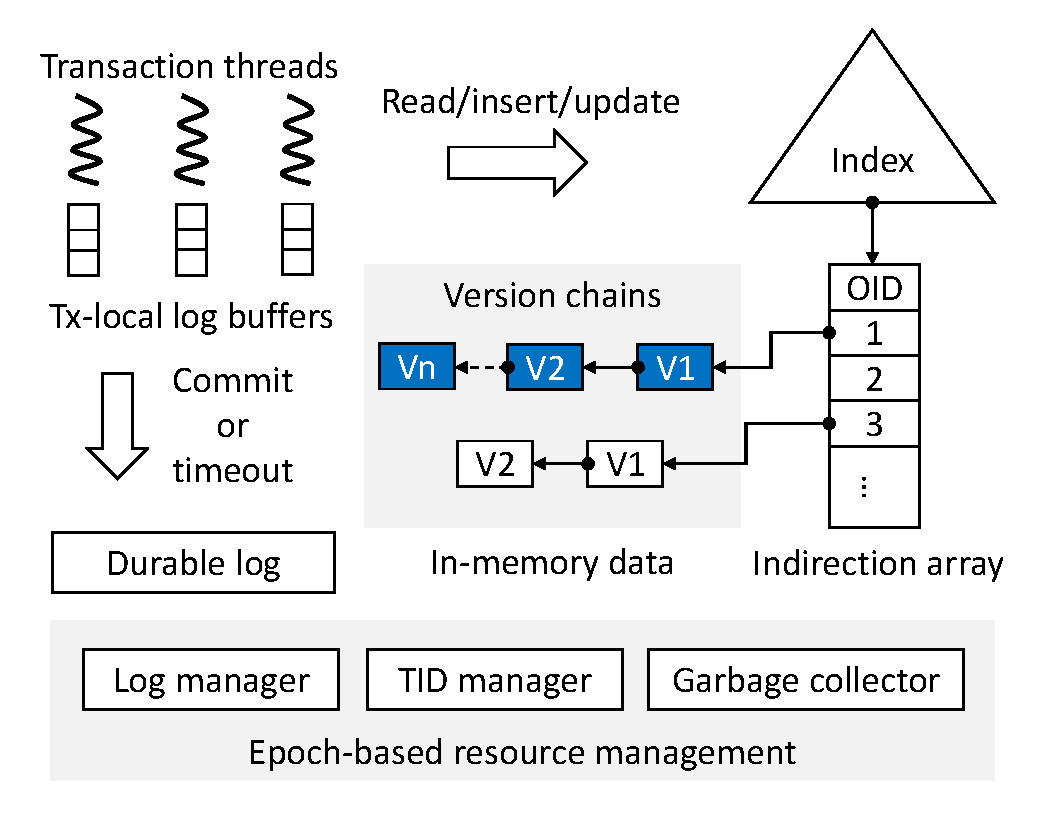
\includegraphics[width=\columnwidth]{ermia-arch}
\caption{Architecture of ERMIA.}
\tianzheng{this diagram fits in \$3 more?}
\end{figure}

\vspace{2mm} 
{\bf Append-only storage.}
Append-only storage allows drastic simplifications of both I/O patterns and corner cases in the code. When combined with a carefully designed log manager and indirection arrays (below), we are able to achieve a single-copy system where the log is a significant fraction of the database (with records graduating from the log to secondary storage only if they go a long time with no updates). The resulting system is also easier to recover, as both undo and redo are largely unnecessary (the log can be truncated at the first hole without losing any committed work).

\vspace{2mm} 
{\bf Logging.}
System designers should also treat recovery as a first class citizen when designing a transaction processing system. Log managers are a well-known source of complexity and bottlenecks in a database system. Many of the recent proposals do not provide thorough design for recovery, at least not even close to the level of details in \cite{MohanHLPS92}.

The in-memory log buffer is a central point of communication that simplifies a variety of other tasks in the system, but which tends to kill scalability. Past work has attempted to optimize \cite{JohnsonPSAA10} or distribute \cite{WangJ14} the log, with partial success and significant additional complexity. Systems such as H-Store \cite{Kallman+08} (and its commercial version, VoltDB) largely dispense with logging and rely instead on replication. These systems replace the logging bottleneck with a transaction dispatch bottleneck. Silo avoids the logging bottleneck by giving up the traditional total order in transactions. Avoiding total ordering is efficient but prevents the system from using any but the simplest of CC schemes---there is no practical way to implement repeatable read or snapshot isolation, for example, and transactions {\it cannot see their own writes without sacrificing performance}.

We advocate a sweet spot between the extremes of fully coordinated logging (multiple synchronization points per transaction) and fully uncoordinated logging (no synchronization at all). A transaction with a reasonably small write footprint should expect to acquire a totally ordered commit timestamp, and reserve all needed space in the log, using a single global atomic operation. Such a system can scale to a few {\em millions} of commits per second \cite{TuZKLM13}---the current world record in TPC-E is not quite 9ktps---while still preserving ordering information that enables advanced concurrency control schemes. We present just such a log manager in \secref{design}.

\vspace{2mm} 
{\bf Concurrency control.} 
Broadly speaking, there are two camps of CC methods: the pessimistic, e.g. two-phase locking (2PL), and the optimistic (OCC). As it has been shown in the past, e.g. \cite{AgrawalCL87}, pessimistic methods theoretically beat optimistic ones under contention, assuming those pessimistic methods can be implemented with sufficiently low overhead relative to their optimistic counterparts. However, in practice this is not easy to achieve. For example, a study of the SHORE storage manager reports roughly 25\% overhead for locking-based pessimistic methods \cite{HarizopoulosAMS08}; that means that any OCC scheme with lower than 25\% abort rate would outperform it.

Having said that, typical memory-optimized engines that employ lightweight OCC and running on modern commodity servers, leave some room for exploration. First, a contentious workload can easily drive abort rates to 25\% or higher, opening the door for more heavyweight schemes. Second, modern systems achieve extraordinarily high throughput for short-running, partition-able transactions with predictable footprints), and it might be worth trading 25\% of peak performance for more robust behavior in a wider spectrum of transactional and mixed workloads. In other words, it is easier to tolerate losing 15-20\% of peak performance if net throughput is still several hundreds of thousands of transactions per second.


There are different flavor of optimistic, or opportunistic, CC. Many recent systems adopt a lightweight validation step at the end of the transaction, during pre-commit. Such kind of validation is very opportunistic, and somewhat brittle, leaving the system vulnerable in many workloads.
Further, these optimistic schemes make no guarantee that it is safe to retry the transaction immediately after pre-commit fails, an issue that performance evaluations often sidestep by not retrying failed transactions at all. Ideally, a good CC scheme would provide a ``safe restart'' property \cite{PortsG12} where the system guarantees that a transaction will not fail twice because of the same conflict.
Regardless optimistic or pessimistic, the CC mechanism should not only have a low false positive rate detecting conflicts, but it should allow the system to detect the glaring conflict cases (cases where a transaction is destined to fail) as early as possible to minimize the amount of wasted work.

At least to our knowledge, there is no (publicly available) system that is both fast enough and has the appropriate infrastructure to support the implementation of robust CC schemes. The infrastructure matters terribly. It decides whether it is even possible to implement a particular CC scheme, and whether that would be practical. For example, the effort to enhance Postgres with serializable snapshot isolation (SSI) required a very large implementation effort, since the team had to integrate what it is essentially a lock manager~\footnote{Once all this groundwork was done, extending Postgres to other CCs is relatively easy.}. And even then, the achieved performance was not impressive, due to severe bottlenecks in multiple parts of the system (the new lock manager and the existing log manager, in particular).  Many of the design decisions we outline in \secref{design} were specifically taken in order to allow more flexibility in implementing multiple CC schemes.

\vspace{2mm}
{\bf Physical layer.} 
The interactions at the physical level are typically handled by a low-level component of any transaction processing system called the storage manager.
The implementation of the storage manager is tightly-coupled to the CC scheme and that makes it difficult to modify or extend the CC of legacy systems.  

In our opinion, one promising technique that provides desirable properties is the indirection array \cite{SadoghiRCB13,Diaconu+13}.
For example, an indirection array reduces the amount of logging required for updates in append-only systems. In a record update only the corresponding entry in the array needs to be updated; without the indirection, creating a new version requires updating every reference to that record, which can be very expensive with tree-based secondary indexes update cascades to the root of every index that has a reference to the changed object, and result cascading updates that may propagate up to the root. Additionally, on record updates the system does not have to update every reference to that record, say from secondary indexes.

As a comparison, Silo does not employ indirection arrays. Instead, it performs in place updates: there is effectively a single committed version of an object with perhaps a private uncommitted copy, unless a special heavyweight snapshot mechanism is invoked. Hekaton is technically multi-versioned, but because of the CC scheme it uses, versions become unusable to non read-only transactions as soon as any overwrite commits. For all practical purposes, both systems are multi-versioned only for read-only transactions.

Indirection arrays are suitable for the physical implementation of CC for multi-versioned systems, as a single compare-and-swap (CAS) operation suffices to install a new version of an object. \kk{ With indirection array as a backing store,  we can install versions without latching overhead minimizing inter-thread communication, and also it allows background reclaiming of old versions without interferring foreground transaction processing as well. }

With indirection arrays, even anti-caching~\cite{DeBrabantPTSZ13} is largely simplified: in the vanilla anti-caching algorithm all the secondary indexes have to be updated, whenever a record is evicted from memory---with some considerable overhead. The indirection array gives a convenient place to replace an in-memory pointer with an on-disk pointer, and in some sense acts as a lightweight buffer pool. 

There are also low-level reasons, detailed in \secref{design:oid}, for using indirection arrays. For example, space management becomes easier, and they admit a convenient analog to cache-friendly compact index structures such as CSB+Trees \cite{RaoR00}. These benefits do not justify adopting indirection, but they become convenient to use once the indirection layer is in place for other reasons.

The flexibility in implementing various CC schemes is greatly enhanced if we can establish total ordering. One way to achieve total ordering, is through a centralized log, which can be used for establishing the transaction commit order. Therefore we opt using a centralized log, but we minimize the interaction with it to only a single communication per transaction. 
In contrast, Silo employs a epoch-based ordering that is only partial. 

